\documentclass[11pt, a4paper]{article}

% --- Essential Packages ---
\usepackage[utf8]{inputenc}
\usepackage[margin=1in]{geometry}
\usepackage{graphicx}
\usepackage{float}
\usepackage{booktabs}
\usepackage{hyperref}
\usepackage{listings}
\usepackage{xcolor}
\usepackage{caption}
\usepackage{multirow}
\usepackage{microtype}
\usepackage{fancyhdr}

% --- Aesthetic Styling ---
\definecolor{accentcolor}{HTML}{D9381E} 
\definecolor{textdark}{HTML}{1A1D20}    
\definecolor{textmuted}{HTML}{5A626D}   

% Page Header/Footer Styling
\pagestyle{fancy}
\fancyhf{}
\fancyhead[L]{\small\color{textmuted}\textbf{A02: Comparative Analysis} | PyTorch vs. TensorFlow}
\fancyhead[R]{\small\color{accentcolor}\textbf{\thepage}}
\renewcommand{\headrulewidth}{0.6pt}
\renewcommand{\headrule}{\hbox to\headwidth{\color{accentcolor}\leaders\hrule height \headrulewidth\hfill}}

\captionsetup{font=small, labelfont={bf, color=accentcolor}}

% --- Code Highlighting Setup ---
\definecolor{codegreen}{rgb}{0,0.5,0}
\definecolor{codegray}{rgb}{0.5,0.5,0.5}
\definecolor{codepurple}{rgb}{0.58,0,0.82}
\definecolor{backcolour}{HTML}{F6F7F9}

\lstdefinestyle{mystyle}{
    backgroundcolor=\color{backcolour},   
    commentstyle=\color{codegreen},
    keywordstyle=\color{accentcolor},
    numberstyle=\tiny\color{codegray},
    stringstyle=\color{codepurple},
    basicstyle=\ttfamily\footnotesize,
    breakatwhitespace=false,         
    breaklines=true,                 
    captionpos=b,                    
    keepspaces=true,                 
    numbers=left,                    
    numbersep=5pt,                  
    showspaces=false,                
    showstringspaces=false,
    showtabs=false,                  
    tabsize=4
}
\lstset{style=mystyle}

% --- Title & Authors ---
\title{\vspace{-1.5cm}\textbf{\huge\color{textdark}A Comparative Analysis of Machine Learning and Deep Learning Tools and Frameworks: PyTorch vs. TensorFlow}}
\author{\large\color{accentcolor}\textbf{DL\_FA2026\_2376\_14562}: Cherluk, Michael, Olubukola, \& Taki \\ \normalsize\color{textmuted}Houston City College -- ITAI 2376}
\date{\small September 3, 2026}

\begin{document}

\maketitle
\vspace{-0.5cm}

\begin{abstract}
\noindent\textbf{\color{accentcolor}Abstract:} This report presents an empirical comparative analysis of two leading deep learning frameworks: PyTorch and TensorFlow. To evaluate architectural performance, resource utilization, and execution speed, we conducted a 10-run controlled benchmark, training identical Convolutional Neural Networks (CNNs) on the MNIST dataset. Both frameworks were evaluated using their respective Just-In-Time (JIT) compilation optimizations (\texttt{torch.compile()} and TensorFlow XLA) to accurately measure steady-state training efficiency. Empirical results indicate performance parity in predictive capability, with both frameworks consistently converging at approximately 98\% test accuracy. However, distinct behavioral variations were observed in raw training time and developer ergonomics. The evidence suggests that neither framework holds universal superiority; rather, the optimal selection depends heavily on the specific research velocity and production deployment constraints of the project.
\end{abstract}

\vspace{0.3cm}

\section{Framework Context Visual}

\begin{figure}[H]
    \centering
    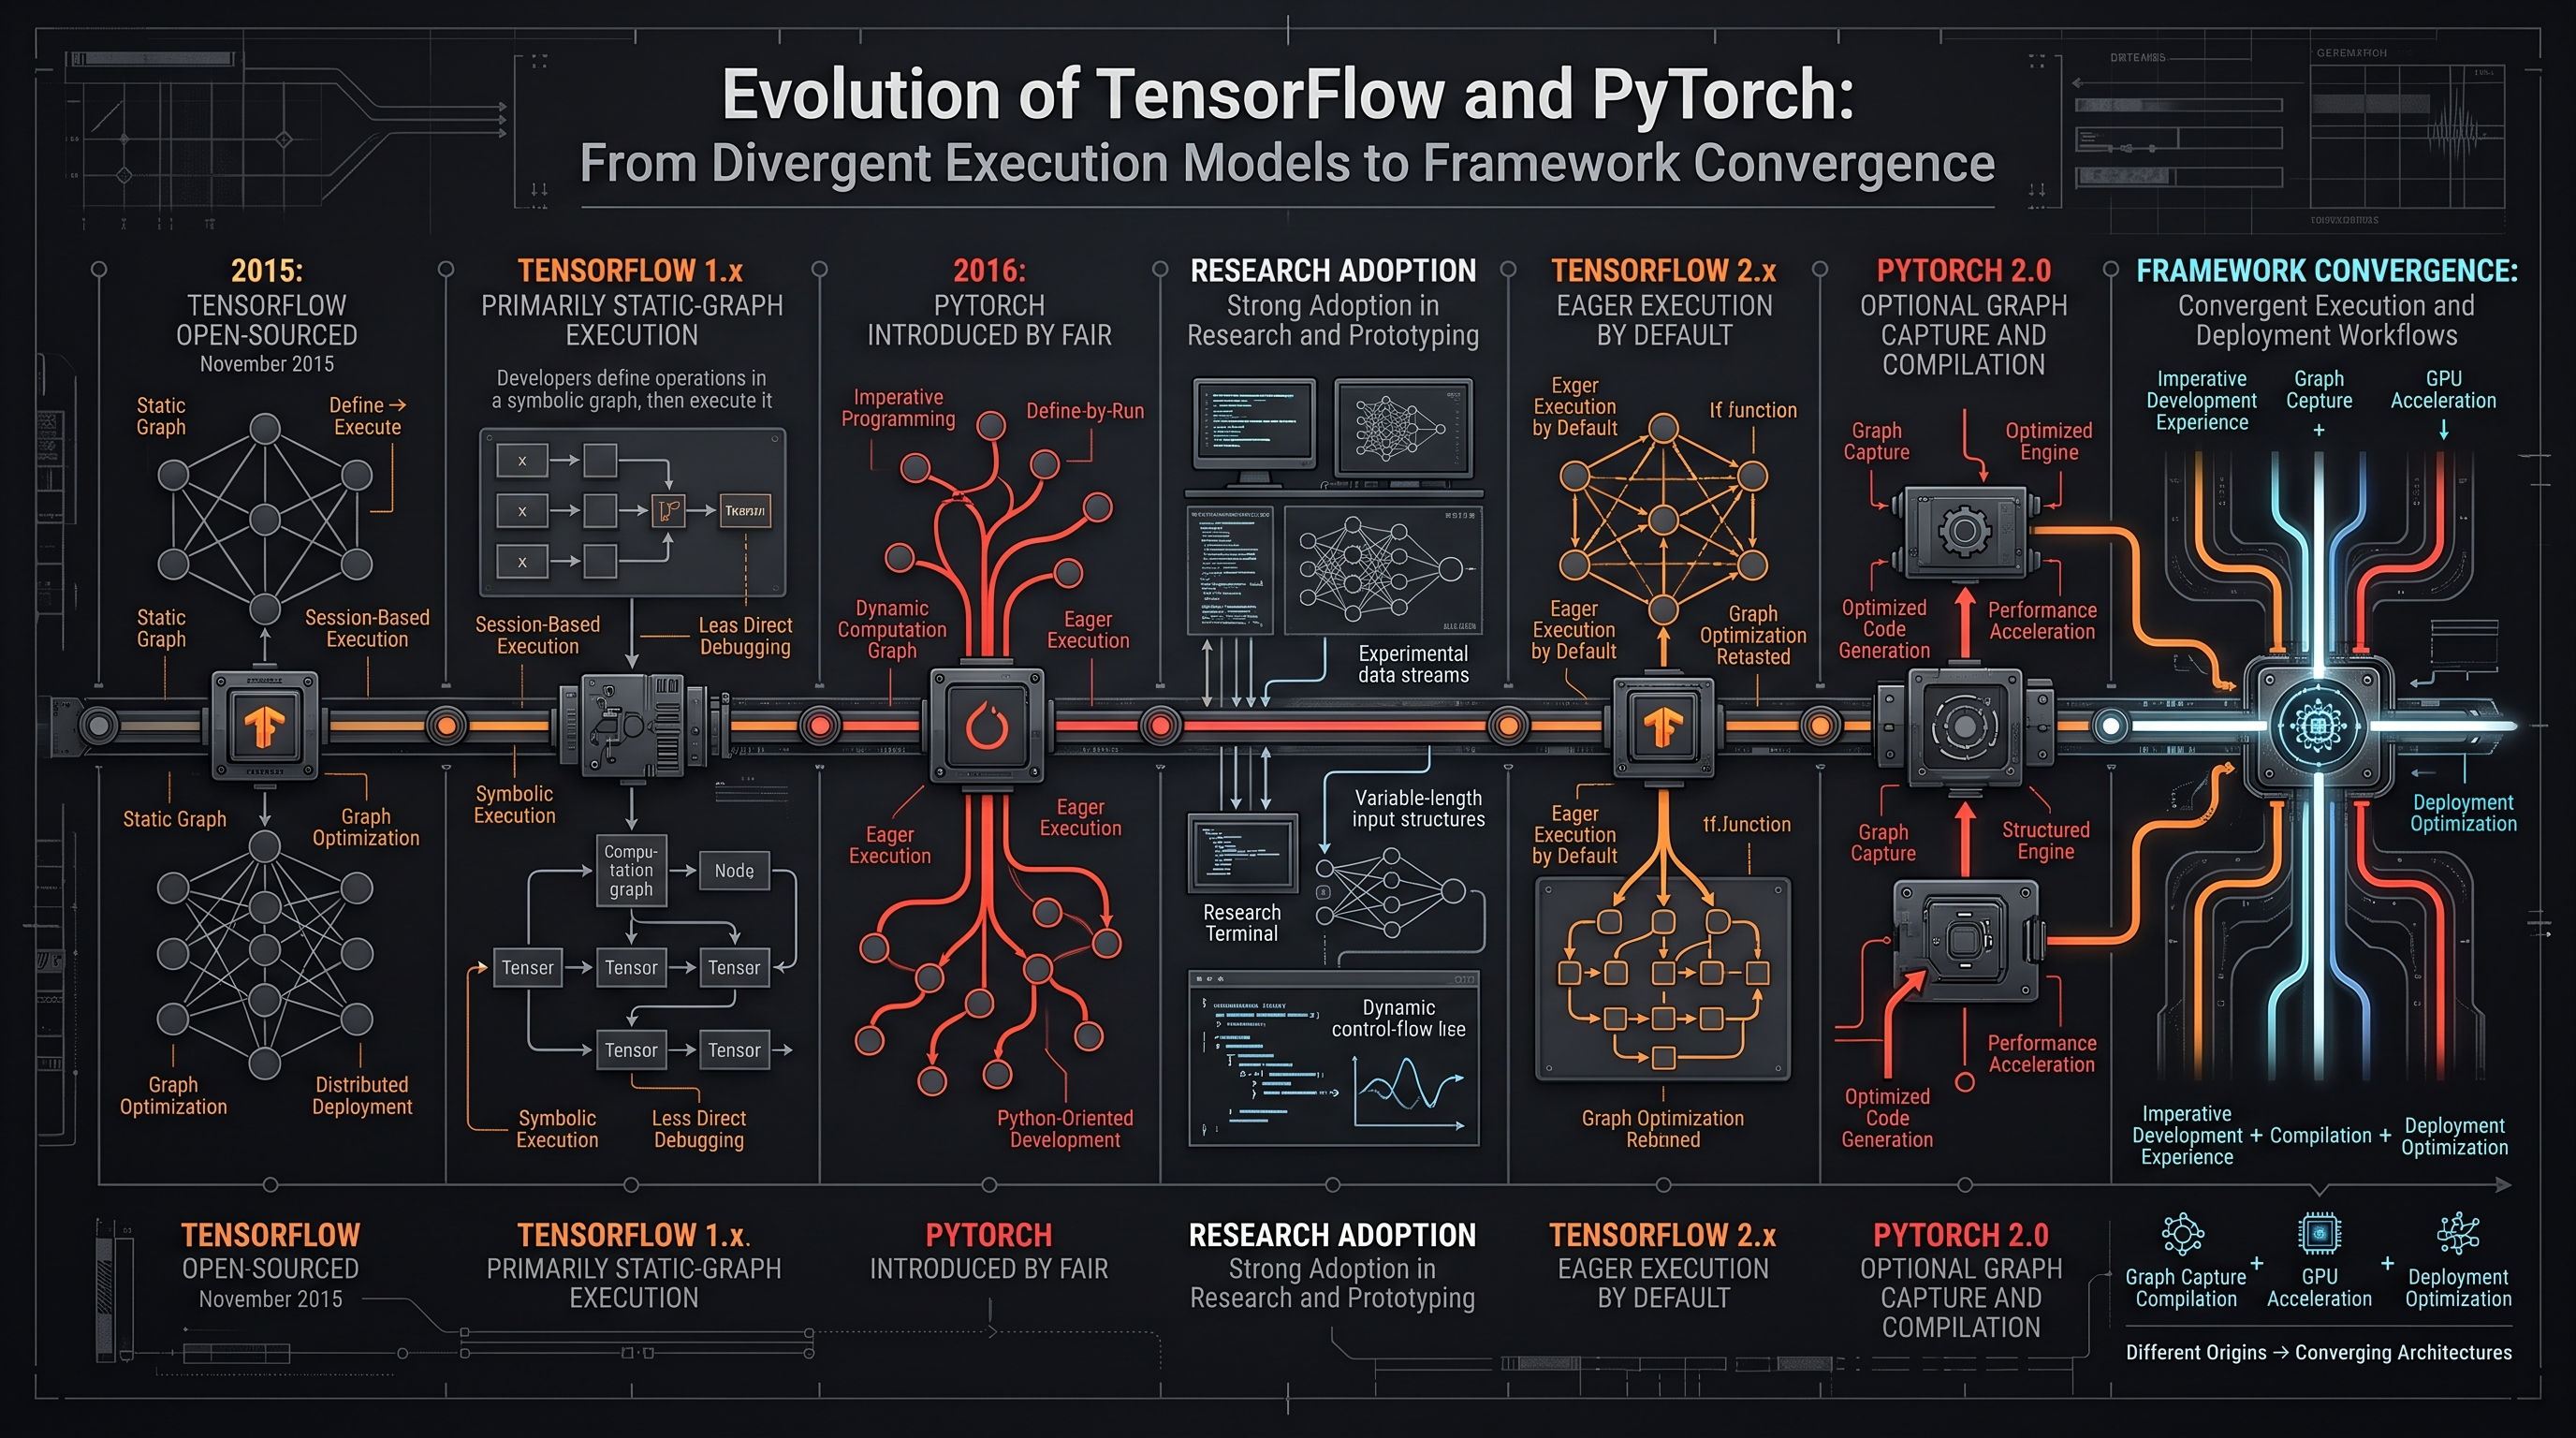
\includegraphics[width=0.9\textwidth]{TimelinePyTorchAndTen.jpeg}
    \caption{Evolution of TensorFlow and PyTorch execution models. TensorFlow 1.x primarily used symbolic static-graph execution, whereas PyTorch was designed around dynamic, eager define-by-run computation. TensorFlow 2.x made eager execution the default, while PyTorch 2.0 added optional graph capture and compilation through \texttt{torch.compile()}.}
    \label{fig:framework_evolution}
\end{figure}

\section{Background: Origin, Development, and Purpose}
The landscape of modern deep learning is defined by two foundational frameworks: TensorFlow and PyTorch. Both were designed to facilitate the rapid development and training of neural networks using GPU acceleration, but they originated from starkly different organizational philosophies and developmental timelines.

TensorFlow was released by Google Brain in November 2015 as an open-source evolution of DistBelief. It was originally built around a static computation graph paradigm (Define-and-Run). Developers had to define the entire mathematical graph before feeding data through it, enabling massive optimization across distributed clusters and edge hardware. However, this abstraction created steep debugging hurdles.

PyTorch was introduced by Meta's AI Research lab (FAIR) in 2016, rooted in the Torch library. It adopted a dynamic computation graph architecture (Define-by-Run) known as Eager Execution, allowing tensors to be evaluated on-the-fly using native Python debuggers. This made PyTorch the premier tool for academic and rapid algorithmic research.

Over time, these frameworks converged: TensorFlow 2.x adopted Eager Execution by default, while PyTorch 2.0 introduced \texttt{torch.compile()} to optimize dynamic graphs for production speed.

\section{Key Features and Advantages}
\begin{itemize}
    \item \textbf{PyTorch}: Features a Pythonic, object-oriented design (\texttt{nn.Module}) that provides granular control over the forward pass. Its primary advantage lies in research velocity, real-time tensor inspection, and seamless integration with standard debugging tools.
    \item \textbf{TensorFlow}: Features robust enterprise deployment tools, high-level abstractions via Keras (\texttt{models.Sequential}), and native multi-platform export capabilities (TensorFlow Lite and TensorFlow Serving), making it ideal for large-scale production scaling.
\end{itemize}

\section{Real-World Applications and Case Studies}
Both frameworks drive critical production systems globally:
\begin{itemize}
    \item \textbf{PyTorch}: Dominates computer vision, natural language processing research, and robotics (such as Tesla's autopilot vision systems and Meta's generative AI infrastructure), where rapid experimentation and custom architectures are paramount.
    \item \textbf{TensorFlow}: Powers large-scale enterprise services (such as Google Translate, Airbnb fraud detection, and Spotify recommendations), where robust microservice deployment and low-latency edge inference are critical.
\end{itemize}

\section{Comparative Perspective: Usability, Performance, and Scalability}
To evaluate architectural performance and execution speed, we conducted a 10-run controlled benchmark, training identical Convolutional Neural Networks (CNNs) on the MNIST dataset using Adam ($lr=0.001$), batch size 64, across 3 epochs.

\begin{table}[H]
    \centering
    \caption{Statistical Summary of Empirical Trials ($N=10$ runs)}
    \label{tab:empirical_stats}
    \begin{tabular}{@{}lcccc@{}}
        \toprule
        \textbf{Framework} & \textbf{Mean} & \textbf{Std Dev} & \textbf{Min} & \textbf{Max} \\
        \midrule
        \multicolumn{5}{c}{\textit{\textbf{Training Time (Seconds)}}} \\
        \midrule
        PyTorch    & 109.6901 & 2.8645 & 106.8112 & 116.0524 \\
        TensorFlow & 185.2347 & 12.5997 & 173.6991 & 213.0359 \\
        \midrule
        \multicolumn{5}{c}{\textit{\textbf{Test Accuracy (\%)}}} \\
        \midrule
        PyTorch    & 98.0540 & 0.1050 & 97.9000 & 98.2400 \\
        TensorFlow & 97.9810 & 0.1570 & 97.7500 & 98.2100 \\
        \bottomrule
    \end{tabular}
\end{table}

\subsection{Usability and Ergonomics}
PyTorch offers superior developer ergonomics due to its intuitive Pythonic syntax and dynamic control flow. TensorFlow, while streamlined via Keras for standard models, introduces debugging complexity when utilizing custom low-level training loops or advanced XLA compilation decorators (\texttt{@tf.function(jit\_compile=True)}).

\subsection{Performance and Scalability}
Empirical data demonstrates that PyTorch's \texttt{torch.compile()} achieved an average training duration of 109.69 seconds with high stability ($\pm 2.86$s), whereas TensorFlow's XLA compilation averaged 185.23 seconds with higher variance ($\pm 12.60$s). Both frameworks achieved predictive parity at ~98\% test accuracy. For enterprise horizontal scaling and serving, TensorFlow maintains a mature microservice ecosystem, whereas PyTorch excels in single-node research velocity and edge-device hardware integration.

\section{Conclusion}
Neither framework holds universal superiority. PyTorch is optimal for research velocity and custom architectural design, while TensorFlow excels in enterprise-scale production deployment.

\newpage
\appendix
\section{Appendix: Benchmarking Script Reference}
\begin{lstlisting}[language=Python, caption=Benchmark Execution Logic]
import matplotlib.pyplot as plt

frameworks = ["PyTorch", "TensorFlow"]
training_times = [pytorch_time, tensorflow_time]
plt.bar(frameworks, training_times)
plt.ylabel("Training Time (seconds)")
plt.title("PyTorch vs TensorFlow Training Time")
plt.show()
\end{lstlisting}

\end{document}
